
\documentclass[twoside,12pt]{article}

\usepackage{dsctemplate}
\usepackage[margin=1in]{geometry}
\usepackage{amsmath}
\usepackage{amssymb,amsthm}
\usepackage{fancyhdr}
\usepackage{nicefrac}
\usepackage{minted}
\usetikzlibrary{quotes,angles,positioning,arrows.meta}
\usetikzlibrary{calc}
\usepackage{enumitem}
\usepackage{fancyvrb}
\usepackage{dirtytalk}
\usepackage{comment}
\usepackage{minted}
\usepackage{emoji}
\usepackage{makecell}
\usepackage{changepage} % for shrinking margins in minipage section

\DefineVerbatimEnvironment{verbatim}{Verbatim}{xleftmargin=.5in}
\newlist{multiplechoice}{itemize}{2}
\setlist[multiplechoice]{label=$\square$}

% configuration
% ------------------------------------------------------------------------------

% control whether solutions are shown or hidden
% \showsolntrue

% page headers only on odd pages
\pagestyle{fancy}
\fancyhead{}
\fancyhead[RO]{uniqname: \rule{3in}{.5pt}}
\renewcommand{\headrulewidth}{0pt}
% \pagenumbering{gobble}

% ------------------------------------------------------------------------------

\begin{document}


\thispagestyle{empty}

\vspace{-5.5in}

\pstitle{%
    Final Exam
}{EECS 398, Winter 2025}

\vspace{-.3in}

\begin{tabular}{rl}
    Full Name: & \inlineresponsebox[4in]{Solutions}\\
    Uniqname: & \inlineresponsebox[4in]{rampure}\\
    UMID: & \inlineresponsebox[4in]{12345678} \vspace{0.2in} \\
    Room: & \bubble{BBB 1670} \bubble{CSRB 2246} \bubble{DOW 1010} \bubble{SSD/Alt} \vspace{.3in} \\ 
\end{tabular}

\vspace{-0.2in}

\hline

\vspace{0.1in}

\textbf{Instructions:}
    \begin{itemize}
       \item You have 120 minutes to complete this exam.
       \item \textbf{This exam consists of 9 questions, worth a total of 100 points.}
        \item Write your uniqname in the top right corner of each page in the space provided.
        \item Please write \textbf{clearly} in the provided answer boxes; we will not grade work that appears elsewhere. Completely fill in bubbles and square boxes; if we cannot tell which option(s) you selected, you may lose points.
        
            \bubble{A bubble means that you should only \textbf{select one choice}.}
            
            \squarebubble{A square box means you should \textbf{select all that apply}. Blank answers will receive no credit.}
            
        \item You may refer to two double-sided handwritten notes sheets. Other than that, you may not refer to any other resources or technology during the exam (no phones, watches, or calculators).
    \end{itemize}

\vspace{.1in}

\hline

\vspace{0.1in}

\noindent You are to abide by the University of Michigan/Engineering Honor Code. To receive a grade,
please sign below to signify that you have kept the Honor Code pledge.

\vspace{0.2in}

\noindent \textit{I have neither given nor received aid on this exam, nor have I concealed any violations of the
Honor Code.}

\vspace{0.2in}

\begin{tabular}{rl}
    \: \: \: \: \: Signature: & \biginlineresponsebox[4in]{}\\
\end{tabular}

\begin{center}

\vspace{-0.05in}

% \huge{Version A}

\end{center}

\newpage

\begin{center}
    \noindent \textbf{\large{Data Overview: Gone Fishin'}}
\end{center}

\noindent In this exam, we'll work with the DataFrame \texttt{fish}, which contains information about various fish for sale at a market in Finland.

\vspace{.1in}

\noindent The first few rows of \texttt{fish} are shown below, but \texttt{fish} has many more rows than are shown.

\begin{center}

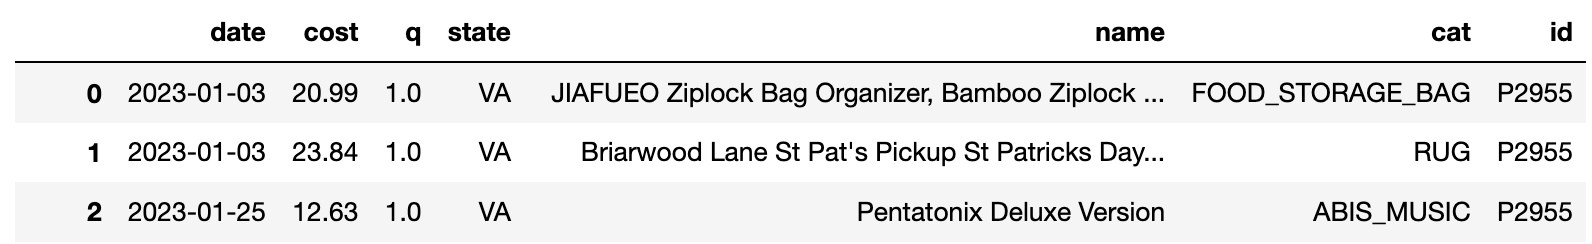
\includegraphics[width=0.4\textwidth]{final-images/df.png}
    
\end{center}

\noindent Each row in \texttt{fish} contains information about a single fish. The columns in \texttt{fish} are as follows:

\begin{itemize}
    \item \texttt{"Height" (float)}: The height of the fish, in inches.
    \item \texttt{"Weight" (float)}: The weight of the fish, in grams.
    \item \texttt{"Species" (str)}: The species of the fish. There are \textbf{7} possible species, 5 of which are shown in the example above.
    \item \texttt{"Width" (float)}: The width of the fish, in inches.
\end{itemize}

\vspace{0.1in}

\noindent Assume that:
\begin{itemize}
    \item All necessary import statements have been run.
    \item Unless otherwise specified, $\lVert \vec v \rVert$ refers to the $L_2$ norm of $\vec v$, i.e. $\lVert \vec v \rVert = \lVert \vec v \rVert_2 = \sqrt{v_1^2 + v_2^2 + ... + v_n^2}$.
    \item If $c \in \mathbb{R}$ is a scalar (i.e. a single number), then $\vec c$ is a vector in which every element is $c$, e.g. $\vec 2$ is a vector of all 2s.
    % \item $I$ represents the identity matrix, which is a square matrix in which the diagonal entries are 1 and all non-diagonal entries are 0.
\end{itemize}

% \noindent As it gets colder outside, it's important to make sure we're taking care of our skin! In this exam, we'll work with the DataFrame \texttt{skin}, which contains information about various skincare products for sale at Sephora, a popular retailer that sells skincare products.

% \vspace{.1in}

% \noindent The first few rows of \texttt{skin} are shown below, but \texttt{skin} has many more rows than are shown.

% % \vspace{-.5in}

% \begin{center}

% 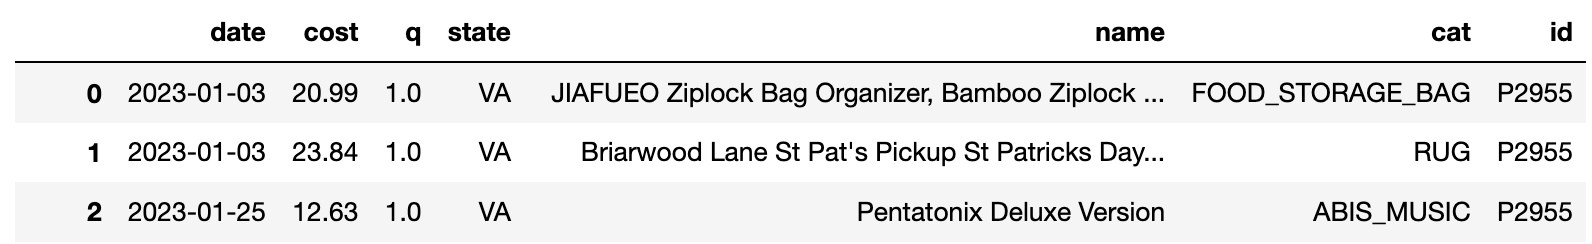
\includegraphics[width=1\textwidth]{final-images/df.png}

% \end{center}

% \vspace{.1in}

% \noindent The columns in \texttt{skin} are as follows:

% \begin{itemize}

% \item{\texttt{"Type" (str)}: The type of product. There are six different possible types, three of which are shown above.}
% \item{\texttt{"Brand" (str)}: The brand of the product. As shown above, brands can have multiple products.}
% \item{\texttt{"Name" (str)}: The name of product. Assume that product names are unique.}
% \item{\texttt{"Price" (int)}: The price of the product, in a whole number of dollars.}
% \item{\texttt{"Rating" (float)}: The rating of the product on \texttt{sephora.com}; ranges from \texttt{0.0} to \texttt{5.0}.}
% \item{\texttt{"Num Ingredients" (int)}: The number of ingredients in the product.}
% \item{\texttt{"Sensitive" (int)}: \texttt{1} if the product is made for individuals with sensitive skin, and \texttt{0} otherwise.}

% \end{itemize}


% \noindent \textbf{Throughout the exam}, assume we have already run all necessary import statements.

\newpage

% \noindent \textbf{Make sure you have read the Data Overview \textit{and} read all of the ques\texttions on the exam before you start writing!}

\begin{probset}

% \begin{prob}

% Suppose we'd like to build a regression model to predict the width of a fish, given various features. Consider the code snippet below.  

% \begin{verbatim}
% fish["1"] = 1
% X_train, X_test, y_train, y_test = train_test_split(
%     fish[["1", "Height", "Weight", "Species"]], fish["Width"]
% )
% model = make_pipeline(
%     make_column_transformer(
%         (OneHotEncoder(drop="first"), ["Species"]),
%         remainder="passthrough" # Keeps the other two features.
%     ),
%     LinearRegression(fit_intercept=False) # We manually created a column of 1s.
% )
% model.fit(X_train, y_train)
% \end{verbatim}

% % Suppose $X_\text{tr}$ and $\vec y_\text{tr}$ represent the design matrix and observation vector from the training set above.

% Suppose the design matrix produced by 

% \begin{subprobset}

% \begin{subprob}
    
% \end{subprob}

% \begin{subprob}

% Which of the following is equivalent to \texttt{model.predict(X\_train)}?

% $$X_\text{tr} (X_\text{tr}^T X_\text{tr})^{-1} X_\text{tr} \vec{y}_\text{tr}$$

% \end{subprob}
    
% \end{subprobset}

% \end{prob}

\begin{prob}[(9 pts)]

Suppose we use the code below to build a multiple linear regression model to predict the width of a fish, given its height and weight.

\begin{verbatim}
X, _, y, _ = train_test_split(fish["Height", "Weight"], fish["Width"])
model = LinearRegression()
model.fit(X, y)

# Used in the grid below.
ws = np.append(model.intercept_, model.coef_)
preds = model.predict(X)
squares = X.shape[0] * mean_squared_error(y, preds)
\end{verbatim}

Assume that:
\begin{itemize}
    \item $X$ and $\texttt{X}$ both represent the design matrix used to train the model, and that \textbf{$X$ is full rank}.
    \item $\vec y$ and $\texttt{y}$ both represent the observation vector used to train the model.
    \item $\vec w^*$ represents the optimal parameter vector found by \texttt{sklearn}.
\end{itemize}

In \textbf{each column} of the grid below, \textbf{select all} mathematical expressions that have the same value as the code expression provided in the column header. The first column has been done for you as an example. Some guidance:

\begin{itemize}
    \item It is possible that some rows are left empty, but there should be at least one square filled in per column. \textit{Tip: Look at one column at a time.}
    \item Assume, just for this part, that $\vec 0$ and $0$ are the same value, e.g. if an expression produces an array of 0s, you would select the $0$ option in the second row.
\end{itemize}

\begin{center}

\[
\begin{array}{|l|c|c|c|c|c|}
\hline
& & a) & b) & c) & d) \\
\hline
& \texttt{X.shape[1]} & \texttt{preds} & \texttt{ws} & \texttt{squares} & \texttt{np.sum(y - preds)} \\[0.2cm]
\hline
\rule{0pt}{0.5cm} 3 & \scalebox{1.3}{$\blacksquare$} & \scalebox{1.3}{$\square$} & \scalebox{1.3}{$\square$} & \scalebox{1.3}{$\square$} & \scalebox{1.3}{$\square$} \\[0.2cm]
\hline
\rule{0pt}{0.5cm} 0 & \scalebox{1.3}{$\square$} & \scalebox{1.3}{$\square$} & \scalebox{1.3}{$\square$} & \scalebox{1.3}{$\square$} & \scalebox{1.3}{$\square$} \\[0.2cm]
\hline
\rule{0pt}{0.5cm} \lVert \vec y - X \vec w^* \rVert^2 & \scalebox{1.3}{$\square$} & \scalebox{1.3}{$\square$} & \scalebox{1.3}{$\square$} & \scalebox{1.3}{$\square$} & \scalebox{1.3}{$\square$}  \\[0.2cm]
\hline
\rule{0pt}{0.5cm} X^TX \vec w^* - X^T \vec y & \scalebox{1.3}{$\square$} & \scalebox{1.3}{$\square$} & \scalebox{1.3}{$\square$} & \scalebox{1.3}{$\square$} & \scalebox{1.3}{$\square$}  \\[0.2cm]
\hline
\rule{0pt}{0.5cm} \vec1^T(\vec y - X \vec w^*) & \scalebox{1.3}{$\square$} & \scalebox{1.3}{$\square$} & \scalebox{1.3}{$\square$} & \scalebox{1.3}{$\square$} & \scalebox{1.3}{$\square$}  \\[0.2cm]
\hline
\rule{0pt}{0.5cm} (X^TX)^{-1}X^T \vec y & \scalebox{1.3}{$\square$} & \scalebox{1.3}{$\square$} & \scalebox{1.3}{$\square$} & \scalebox{1.3}{$\square$} & \scalebox{1.3}{$\square$}  \\[0.2cm]
\hline
\rule{0pt}{0.5cm} X(X^TX)^{-1}X^T \vec y & \scalebox{1.3}{$\square$} & \scalebox{1.3}{$\square$} & \scalebox{1.3}{$\square$} & \scalebox{1.3}{$\square$} & \scalebox{1.3}{$\square$}  \\[0.2cm]
\hline
\end{array}
\]

\end{center}
    
\end{prob}

\newpage

\begin{prob}[(5 pts)]

Suppose we'd like to build a regression model to predict the width of a fish, given its height and weight.

\begin{subprobset}
    
\begin{subprob}(3 pts) For each of several model instances, we train a model twice --- once with the features as-is, and once with standardized features. In other words:

\begin{verbatim}
# Without standardization
model = ModelClass() # e.g. model = Lasso(alpha=10000)
model.fit(X, y)

# With standardization
model_std = make_pipeline(StandardScaler(), ModelClass())
model_std.fit(X, y)
\end{verbatim}

We say a model is \textbf{standardization invariant} if its training mean squared error is \textbf{guaranteed} to be the same, with or without standardization. Which of the models below are standardization invariant? \textbf{Select all} that apply.

\squarebubble{\texttt{LinearRegression()}}

\squarebubble{\texttt{Ridge(alpha=10)}}

\squarebubble{\texttt{Lasso(alpha=1)}}

\squarebubble{\texttt{Lasso(alpha=10000)}}

\squarebubble{\texttt{DecisionTreeRegressor(max\_depth=3)}}

\squarebubble{\texttt{KNeighborsRegressor(n\_neighbors=5)}}

\squarebubble{\texttt{KNeighborsRegressor(n\_neighbors=8)}}

\end{subprob}

\vspace{0.2in}

\begin{subprob}(2 pts) Consider the two model instances below.

\begin{verbatim}
once = make_pipeline(StandardScaler(), ModelClass())
twice = make_pipeline(StandardScaler(), StandardScaler(), ModelClass())
\end{verbatim}

True or False: As long as \texttt{ModelClass()} is a valid regression model in \texttt{sklearn} that behaves deterministically*, \texttt{once} and \texttt{twice} are \textbf{guaranteed} to have the same training mean squared error.

\bubble{True} 

\bubble{False}

\textit{\small{*By this, we mean that the model makes the same predictions every time it is fit on the same training set. Technically, not all models behave this way.}}


\end{subprob}

\end{subprobset}

\end{prob}

\newpage

\begin{prob}[(6 pts)]

Suppose $A \in \mathbb{R}^{n \times d}$ is a matrix, $\vec b \in \mathbb{R}^n$ is a vector, $\theta$ is a \textbf{negative} number, and that $\vec v^*$ is \textbf{a} vector that minimizes $\lVert \vec b - A \vec v \rVert^2$. In other words: $$\vec v^* = \underset{\vec v}{\text{argmin}} \lVert \vec b - A \vec v \rVert$$

Furthermore, suppose that one of the columns in $A$ is $\vec \theta = \begin{bmatrix} \theta \\ \theta \\ \vdots \\ \theta\end{bmatrix}$.

\begin{subprobset}

\begin{subprob}(3 pts) What is the value of $\vec \theta^T (\vec b - A \vec v^*)$?

\bubble{$0$}

\bubble{$\vec 0$} 

\bubble{$1$} 

\bubble{$\vec 1$} 

\bubble{$\theta$} 

\bubble{$\vec \theta$} 

\bubble{None of these}
    
\end{subprob}

\vspace{0.2in}

\begin{subprob}(3 pts) Select the true statement below.

\textit{Hint: Remember that $\theta$ is a \textbf{negative} number, $n$ is the number of rows in $A$, and $I$ is the identity matrix, a square matrix in which the diagonal entries are 1 and all non-diagonal entries are 0.}

\bubble{If $A^TA - n \theta I$ is invertible, then the value of $\vec v^*$ is unique.}

\bubble{If $A^TA + n \theta I$ is invertible, then the value of $\vec v^*$ is unique.}

\bubble{If $A^TA + n \theta I$ is \textbf{not} invertible, then the value of $\vec v^*$ is \textbf{not} unique.}

\bubble{If the value of $\vec v^*$ is unique, then $A^TA + n \theta I$ is invertible.}

\bubble{If the value of $\vec v^*$ is unique, then $A^TA + n \theta I$ is \textbf{not} invertible.}

\end{subprob}
    
\end{subprobset}
    
\end{prob}

\newpage

\begin{prob}[(14 pts)]

Suppose we'd like to build a regression model to predict the width of a fish, given its height, weight, and species. Consider the following two possible approaches to building linear regression models:

\begin{itemize}
\item \textbf{Approach 1}: One hot encode species using \texttt{OneHotEncoder(drop="first")}, use height and weight as-is, and fit a linear regression model.
\item \textbf{Approach 2}: Fit 7 separate sub-models, one for each unique value of species, where each sub-model is a linear regression model that uses height and weight only.

    \begin{itemize}

    \item For instance, one of the 7 sub-models would be for the Perch species; we'd query the training data to keep only the rows corresponding to the species Perch, then fit the Perch sub-model on just this subset of the training data. 
    
    \item To predict the width of a new fish, we use the sub-model corresponding to the new fish's species.
    
    \end{itemize}

Assume that in \textbf{both} approaches, the linear regression models being considered include \textbf{intercept terms}.

\end{itemize}

\begin{subprobset}

\begin{subprob}(2 pts) Suppose the mean squared error on the training set for approaches 1 and 2 are $\text{MSE}_1$ and $\text{MSE}_2$, respectively. Fill in the \boxed{???}: 

$$\displaystyle \text{MSE}_1 \:\:\: \boxed{???} \:\:\: \text{MSE}_2$$

\bubble{$\geq$} 

\bubble{$>$} 

\bubble{$=$} 

\bubble{$<$} 

\bubble{$\leq$} 

\bubble{Impossible to tell} 

\end{subprob}

\vspace{0.2in}

\begin{subprob}(6 pts) Suppose we visualize both models in 3 dimensions, where one axis represents height, one axis represents weight, and one axis represents predicted width.

\vspace{0.1in}

Fill in the blanks: In the 3 dimensional space described above, 

the fit model in \textbf{approach 1} looks like \_\_(i)\_\_ \_\_(ii)\_\_ \_\_(iii)\_\_,

while the fit model in \textbf{approach 2} looks like \_\_(iv)\_\_ \_\_(v)\_\_ \_\_(vi)\_\_.

\vspace{0.1in}

TODO add the options

\end{subprob}

\end{subprobset}

\newpage

It is possible to construct a design matrix $X'$ such that approach 2 is implemented as a single linear regression model, rather than 7 separate linear regression models.

\begin{subprobset}

\begin{subprob}(2 pts) How many columns are in the design matrix, $X'$? 

% \textit{Hint: This design matrix \textbf{should not} have a column of all 1s.}

\inlineresponsebox[2in]{}

\end{subprob}

\vspace{0.2in}

\begin{subprob}(4 pts) In 1-2 English sentences, describe how to create $X'$. Then, sketch an example of how $X'$ might look, including at least two example rows, one of which should correspond to a fish of the Perch species with a height of 50 and weight of 25. Feel free to use ellipses, ..., in your answer.

\begin{responsebox}{5.5in}

\end{responsebox}
    
\end{subprob}

\end{subprobset}

\end{prob}

\newpage

\begin{prob}[(14 pts)]

Suppose we'd like to build a regression model to predict the width of a fish, given various features. Consider the six line graphs shown below.

\begin{center}

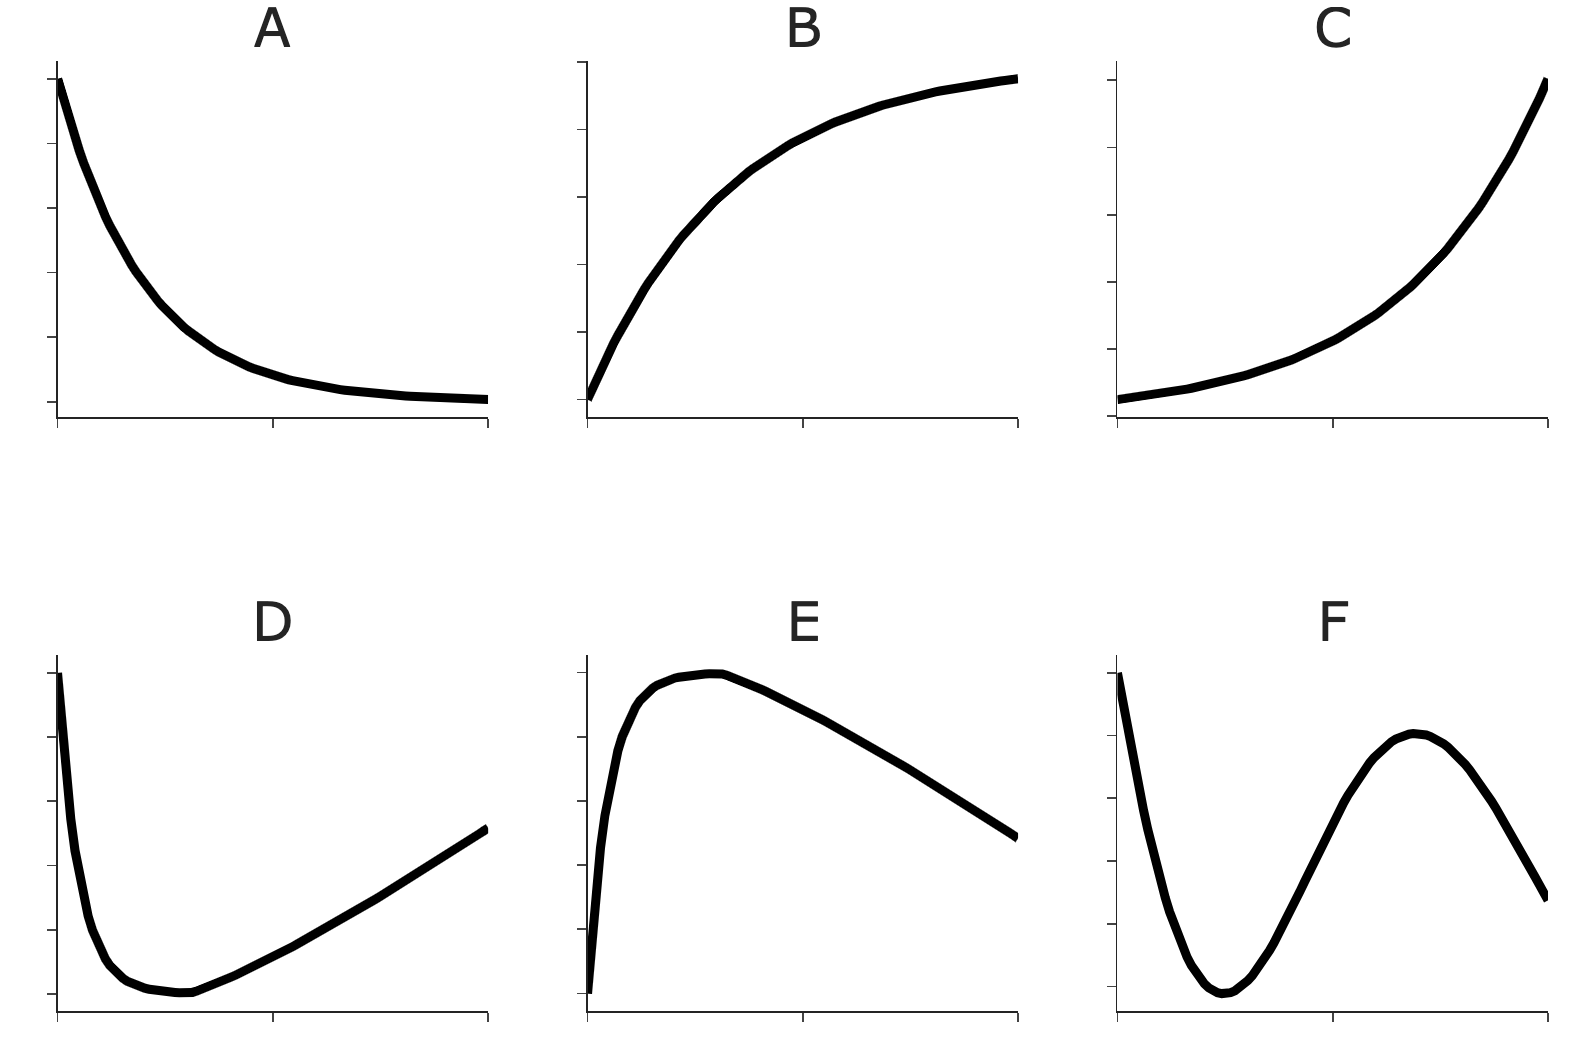
\includegraphics[width=0.6\textwidth]{final-images/curves.png}
    
\end{center}

% Each part below describes a graph of the form $y$ vs. $x$, where $y$ represents a measurement of model performance and $x$ represents a hyperparameter. 

In each part, select the graph that \textbf{best} represents the relationship between model performance (drawn on the $y$-axis) and the provided hyperparameter (drawn on the $x$-axis).

% For instance, in part (a), we are referring to a graph that has training mean squared error on the $y$-axis, and $k$ on the $x$-axis. 

First, suppose we build a \textbf{$k$-nearest neighbors regression} model, as seen in Homework 8.

\begin{subprobset}

\begin{subprob}(2 pts) Which graph best represents \textbf{training mean squared error} ($y$-axis)

vs. $k$ ($x$-axis)?

\bubble{A}

\bubble{B}

\bubble{C}

\bubble{D}

\bubble{E}

\bubble{F}

\end{subprob}

\begin{subprob}(2 pts) Which graph best represents \textbf{test set mean squared error} vs. $k$?

\bubble{A}

\bubble{B}

\bubble{C}

\bubble{D}
    
\bubble{E}

\bubble{F}

\end{subprob}

\begin{subprob}(2 pts) Which graph best represents \textbf{model variance} vs. $k$?

\bubble{A}

\bubble{B}

\bubble{C}

\bubble{D}
    
\bubble{E}

\bubble{F}
    
\end{subprob}

\end{subprobset}

Now, suppose we build a \textbf{linear regression model with degree-$d$ polynomial features}.

\begin{subprobset}

\begin{subprob}(2 pts) Which graph best represents \textbf{training mean squared error} vs. $d$?

\bubble{A}

\bubble{B}

\bubble{C}

\bubble{D}
    
\bubble{E}

\bubble{F}

\end{subprob}

\begin{subprob}(2 pts) Which graph best represents \textbf{test set $R^2$} vs. $d$? \textit{Hint: Recall from Homework 8, $0 \leq R^2 \leq 1$, where larger values of $R^2$ indicate better predictions.}

\bubble{A}

\bubble{B}

\bubble{C}

\bubble{D}
    
\bubble{E}

\bubble{F}
    
\end{subprob}

\begin{subprob}(2 pts) Which graph best represents \textbf{model variance} vs. $d$?

\bubble{A}

\bubble{B}

\bubble{C}

\bubble{D}
    
\bubble{E}

\bubble{F}

\end{subprob}

\end{subprobset}

Finally, suppose we build a \textbf{ridge regression model with hyperparameter $\lambda$}.

\begin{subprobset}

\begin{subprob}(2 pts) Which graph best represents \textbf{model variance} vs. $\lambda$?

\bubble{A}

\bubble{B}

\bubble{C}

\bubble{D}
    
\bubble{E}

\bubble{F}
    
\end{subprob}
    
\end{subprobset}

\end{prob}

\newpage

\begin{prob}[(9 pts)]

Suppose we'd like to build a $L_1$-regularized (LASSO) regression model to predict the width of a fish, given its height and weight. To choose a value of $\lambda$ (the regularization hyperparameter) from the list $[0.01, 0.1, 1, 10]$, we perform $k$-fold cross-validation with $k=4$.


\begin{subprobset}

\begin{subprob}(3 pts) Consider the following optimal parameter vectors, each of which came from minimizing $L_1$-regularized empirical risk using a different value of $\lambda$. 

(In each parameter vector, the 0th component represents the intercept term, the 1st component represents the coefficient on height, and the 2nd component represents the coefficient on weight.)

$$
\vec{w}_a^* = \begin{bmatrix} 2.6999 \\ 0.0105 \\ 0.0041 \end{bmatrix} \qquad
\vec{w}_b^* = \begin{bmatrix} 3.0674 \\ 0.0000 \\ 0.0034 \end{bmatrix} \qquad
\vec{w}_c^* = \begin{bmatrix} 2.0728 \\ 0.1236 \\ 0.0031 \end{bmatrix}
$$

\begin{enumerate}[label=(\roman*)]
    \item Which optimal parameter vector resulted from choosing $\lambda = 0.01$? 
    
    \bubble{$\vec w_a^*$} \bubble{$\vec w_b^*$} \bubble{$\vec w_c^*$}
    
    \item Which optimal parameter vector resulted from choosing $\lambda = 0.1$? 
    
    \bubble{$\vec w_a^*$} \bubble{$\vec w_b^*$} \bubble{$\vec w_c^*$}
    
    \item Which optimal parameter vector resulted from choosing $\lambda = 1$?
    
    \bubble{$\vec w_a^*$} \bubble{$\vec w_b^*$} \bubble{$\vec w_c^*$}
    
\end{enumerate}
    
\end{subprob}

\vspace{0.05in}

\begin{subprob}(3 pts) Suppose, just for this part, that:

\begin{itemize}
    \item Our entire dataset has $N$ rows.
    \item To split the dataset of $N$ rows into training and test sets, we use \texttt{train\_test\_split} with \texttt{test\_size=0.2}.
\end{itemize}

While performing 4-fold cross-validation, each time a model is trained, 90 points are used to train the model. What is the value of $N$?

\bubble{100} 

\bubble{108} 

\bubble{120} 

\bubble{150} 

\bubble{180} 

\bubble{None of these}
    
\end{subprob}

\vspace{0.05in}

\begin{subprob}(3 pts) Average validation mean squared errors are shown in the table below.

\begin{center}

\begin{array}{|c|c|c|c|c|} 
\hline
& \text{Fold 1} & \text{Fold 2} & \text{Fold 3} & \text{Fold 4} \\ 
\hline
\lambda = 0.01 & 15 & 9 & 12 & 12 \\ 
\hline
\lambda = 0.1 & 12 & 18 & 6 & 12 \\ 
\hline
\lambda = 1 & 3 & 12 & 15 & m \\ 
\hline
\lambda = 10 & 18 & 6 & 3 & 9 \\ 
\hline
\end{array}

\end{center}

Given that $\lambda = 1$ is the hyperparameter with the best cross-validation performance above, provide the best possible upper-bound for a value of $m$. That is, find $M$ such that, as long as $m < M$, $\lambda = 1$ is the best choice of $\lambda$. Give your answer as a \textbf{constant with no variables}.

\vspace{0.1in}

\biginlineresponsebox[2in]{}
    
\end{subprob}
    
\end{subprobset}
    
\end{prob}

\newpage

\begin{prob}[(12 pts)]

Let $\vec x = \begin{bmatrix} x_1 \\ x_2 \end{bmatrix}$. Consider the function $f(\vec x) = (x_1^2 + x_2 - 3)^2 + (x_1 + x_2^2 - 4)^2$.

\begin{subprobset}

\begin{subprob}(6 pts) $\nabla f(\vec x)$, the gradient of $f$, can be written in the form $\boxed{\nabla f(\vec x) = A \vec g}$, where $A \in \mathbb{R}^{2 \times 2}$ and $\vec g \in \mathbb{R}^2$. Fill in the blanks to complete the definitions of $A$ and $\vec g$. All blanks should be filled with expressions involving $x_1$, $x_2$, and/or constants.

$$A = \begin{bmatrix} 2x_1 & \_\_(\text{i})\_\_ \\ 1 & \_\_(\text{ii})\_\_ \end{bmatrix} \qquad \qquad \vec g = 2\begin{bmatrix} \_\_(\text{iii})\_\_  \\ \_\_(\text{iv})\_\_ \end{bmatrix} $$

\begin{tabular}{ll}
\text{(i) \hspace{0.0002in}}: \inlineresponsebox[2.75in]{} & (iii): \inlineresponsebox[2.75in]{} \\
(ii): \inlineresponsebox[2.75in]{} & (iv): \inlineresponsebox[2.75in]{} \\
\end{tabular}
    
\end{subprob}

\begin{subprob}(4 pts) We'd like to use gradient descent to minimize $f$. We choose an initial guess of $\vec x^{(0)} = \begin{bmatrix} 1 \\ 0 \end{bmatrix}$ and learning rate/step size $\beta$. Given that $A = \begin{bmatrix} 2 & 1 \\ 1 & 0 \end{bmatrix}$ and $\vec g = \begin{bmatrix} -4 \\ -6 \end{bmatrix}$ when evaluated on $\vec x^{(0)}$, perform one iteration of gradient descent. In other words, what is $\vec x^{(1)}$?

Show your work, and put a $\boxed{\text{box}}$ around your final answer, which should be a vector with two components, both of which are expressions involving $\beta$ and/or constants, but no other variables (i.e. $x$ should not appear in your answer).

\begin{responsebox}{2.5in}
    
\end{responsebox}
    
\end{subprob}

\begin{subprob}(2 pts) Suppose $Q(\vec x)$ is a convex function. True or False: Given that gradient descent converges to the global minimum of $Q$ in $T$ iterations, it is guaranteed that:

\vspace{-0.1in}

$$\lVert \vec x^{(1)} - \vec x^{(0)} \rVert > \lVert \vec x^{(t+1)} - \vec x^{(t)} \rVert, \:\:\: \text{for } t = 1, 2, ..., T-1$$

\bubble{True} 

\bubble{False}

\end{subprob}
    
\end{subprobset}

\end{prob}

\newpage

% \begin{prob}

% Suppose we build a logistic regression model to predict whether a fish is of species \texttt{"Bream"} (class 1) or not (class 0), using $d$ features. The true labels and predicted probabilities for a 12-row training set are shown below; note that the true label is unknown for one of the observations.

% \vspace{-0.1in}

% \begin{center}
% \begin{tabular}{cc}
% \toprule
% \textbf{True Label, $y_i$} & \textbf{Predicted Probability, $P(y_i = 1 | \vec x_i)$}\\
% \midrule
% 0 & 0.90\\
% 1 & 0.85\\
% 1 & 0.85\\
% 1 & 0.62\\
% 0 & 0.62\\
% 1 & 0.55\\
% ??? & 0.55\\
% 0 & 0.55\\
% 1 & 0.33\\
% 0 & 0.25\\
% 0 & 0.24\\
% 0 & 0.19\\
% \bottomrule
% \end{tabular}
% \end{center}

% \vspace{-0.1in}

% Once we fix a classification threshold $T$, where $0 \leq T \leq 1$, we classify fish as follows:

% $$\text{predicted class}_i = \begin{cases} 1 & P(y_i = 1 | \vec x_i) \geq T \\ 0 & P(y_i = 1 | \vec x_i) < T \end{cases}$$

% \begin{subprobset}

% \begin{subprob}

% Among the options below, what is the largest threshold $T_\text{recall-max}$ such that the classifier achieves a recall of 1 (100\%) on the training set?   

% \bubble{$0.23$} \bubble{$0.26$} \bubble{$0.32$} \bubble{$0.34$} \bubble{$0.44$} \bubble{$0.45$}

% \end{subprob}

% \begin{subprob}

% Suppose we choose the threshold $T = 0.5$. Which of the following options accurately describe a \textbf{possible} combination of our classifier's precision, recall, and accuracy? Select all that apply.

% \squarebubble{Precision: $1 / 2$, Recall: $4/5$, Accuracy: $2/3$}

% \correctsquarebubble{Precision: $1/2$, Recall: $4/5$, Accuracy: $7/12$}

% \squarebubble{Precision: $1 / 2$, Recall: $5/6$, Accuracy: $2/3$}

% \squarebubble{Precision: $4/5$, Recall: $5/8$, Accuracy: $7/12$}

% \squarebubble{Precision: $4/5$, Recall: $4/5$, Accuracy: $2/3$}

% \squarebubble{Precision: $4/5$, Recall: $1/2$, Accuracy: $7/12$}

% \squarebubble{Precision: $5/8$, Recall: $4/5$, Accuracy: $2/3$}

% \squarebubble{Precision: $5/8$, Recall: $4/5$, Accuracy: $7/12$}

% \correctsquarebubble{Precision: $5/8$, Recall: $5/6$, Accuracy: $2/3$}
    
% \end{subprob}

% \end{subprobset}

% \newpage

% For your convenience, the same training set from the previous page is shown again below.

% \begin{center}
% \begin{tabular}{llr}
% \toprule
% \textbf{True Label, $y_i$} & \textbf{Predicted Probability, $P(y_i = 1 | \vec x_i)$}\\
% \midrule
% 0 & 0.90\\
% 1 & 0.85\\
% 1 & 0.85\\
% 1 & 0.62\\
% 0 & 0.62\\
% 1 & 0.55\\
% ??? & 0.55\\
% 0 & 0.55\\
% 1 & 0.33\\
% 0 & 0.25\\
% 0 & 0.24\\
% 0 & 0.19\\
% \bottomrule
% \end{tabular}
% \end{center}

% \begin{subprobset}

% \begin{subprob}

% % Recall, our logistic regression model predicts probabilities according to:

% % $$P(y_i = 1 | \vec x_i) = \sigma(w_0^* + w_1^* x_i^{(1)} + w_2^* x_i^{(2)} + ... + w_d^* x_i^{(d)})$$

% % where $w_0^*, w_1^*, ..., w_d^*$ are chosen to minimize empirical risk.

% Suppose our logistic regression model used $d=1$ feature to predict probabilities. Select the true statement below.

% \bubble{The training set above is linearly separable.}

% \bubble{The training set above might be linearly separable.}

% \bubble{The training set above is not linearly separable.}

% \end{subprob}

% \begin{subprob}

% Suppose our logistic regression model used $d=2$ features to predict probabilities. Select the true statement below.

% \bubble{The training set above is linearly separable.}

% \bubble{The training set above might be linearly separable.}

% \bubble{The training set above is not linearly separable.}

% \end{subprob}

% \begin{subprob}

% True or False: If there exists some decision tree that can achieve 100\% training accuracy on some training set, then that training set must be linearly separable.

% \bubble{True} \bubble{False}
    
% \end{subprob}

% \begin{subprob}

% In one English sentence, describe \textbf{exactly one} reason why we prefer cross-entropy loss over squared loss when finding optimal model parameters for logistic regression.

% \begin{responsebox}{1.5in}
    
% \end{responsebox}

% \end{subprob}

% \end{subprobset}

% \end{prob}

\newpage

\begin{prob}[(20 pts)]

Suppose we build a classifier to predict whether a fish is of species Bream (class 1) or not (class 0), given its height and/or weight.

Consider the training set of $n=40$ points below. Note that the 10 points in black correspond to class 1, and the 30 \boxed{\text{outlined}} points correspond to class 0. Assume there are no black points hidden under outlined points and vice versa.

\begin{center}
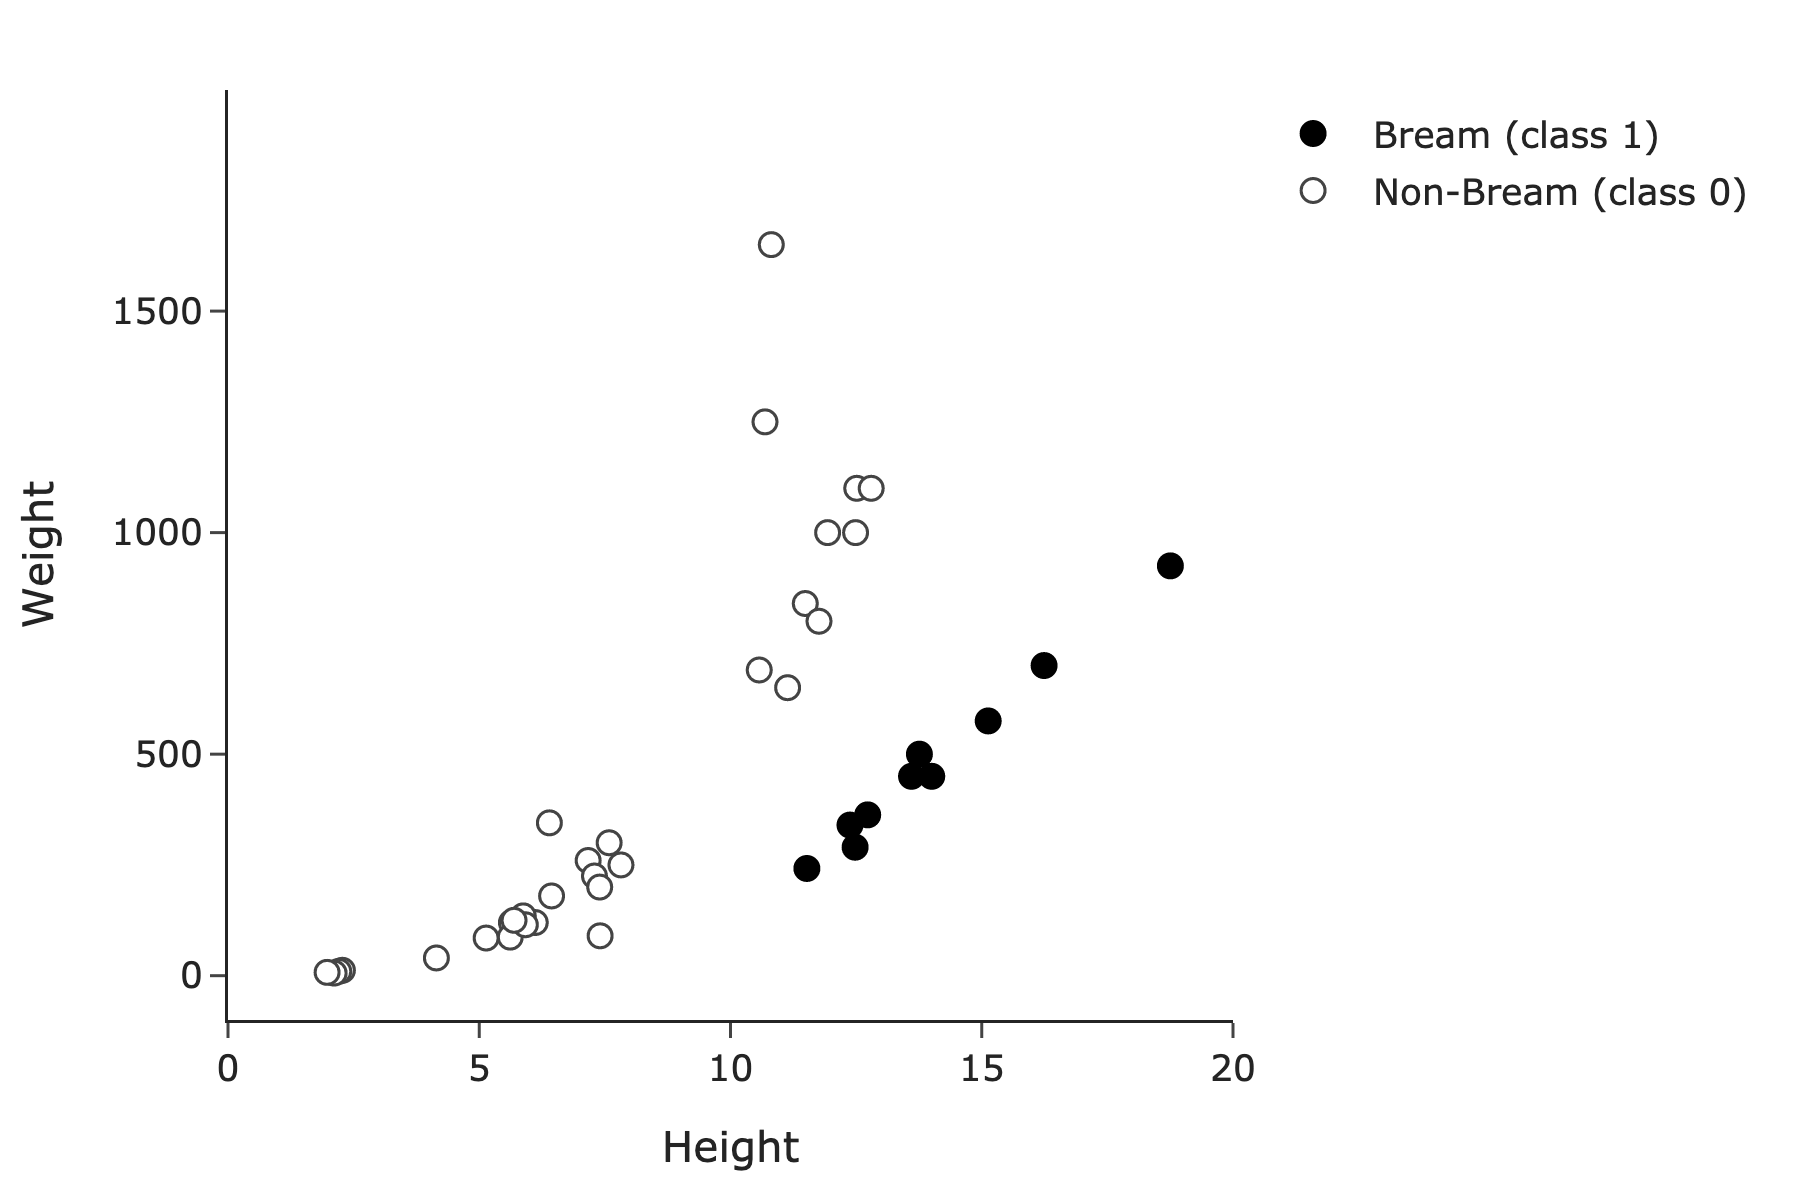
\includegraphics[width=0.8\textwidth]{final-images/scatter-base.png}
\end{center}

\begin{subprobset}

\begin{subprob}(1 pt) Suppose we use height \textbf{only} to predict species. In the 1-dimensional feature space, is the training set linearly separable?

\bubble{Yes} 

\bubble{No}
    
\end{subprob}

\vspace{0.2in}

\begin{subprob}(1 pt) Suppose we use \textbf{both} height and weight to predict species. In the 2-dimensional feature space, is the training set linearly separable?

\bubble{Yes} 

\bubble{No}
    
\end{subprob}

\vspace{0.2in}

\begin{subprob}(3 pts) Suppose we use \textbf{both} height and weight to predict species. What is \textbf{minimum} depth $d$ required for a decision tree classifier to achieve a training accuracy of 100\%?

\bubble{1} 

\bubble{2} 

\bubble{3} 

\bubble{4} 

\bubble{5} 

\bubble{10} 

\bubble{40}

\end{subprob}

\vspace{0.2in}

\begin{subprob}(2 pts) Suppose we use \textbf{both} height and weight to predict species. If we use a $k$-nearest neighbors classifier with $k=1$, which class would be predicted for a fish with height 20 and weight 1250?

\bubble{Class 1 (Bream)} 

\bubble{Class 0 (non-Bream)}
    
\end{subprob}

\end{subprobset}

\newpage

For your convenience, we show the training set of $n=40$ points again below, in which 10 points belong to class 1.

\begin{center}
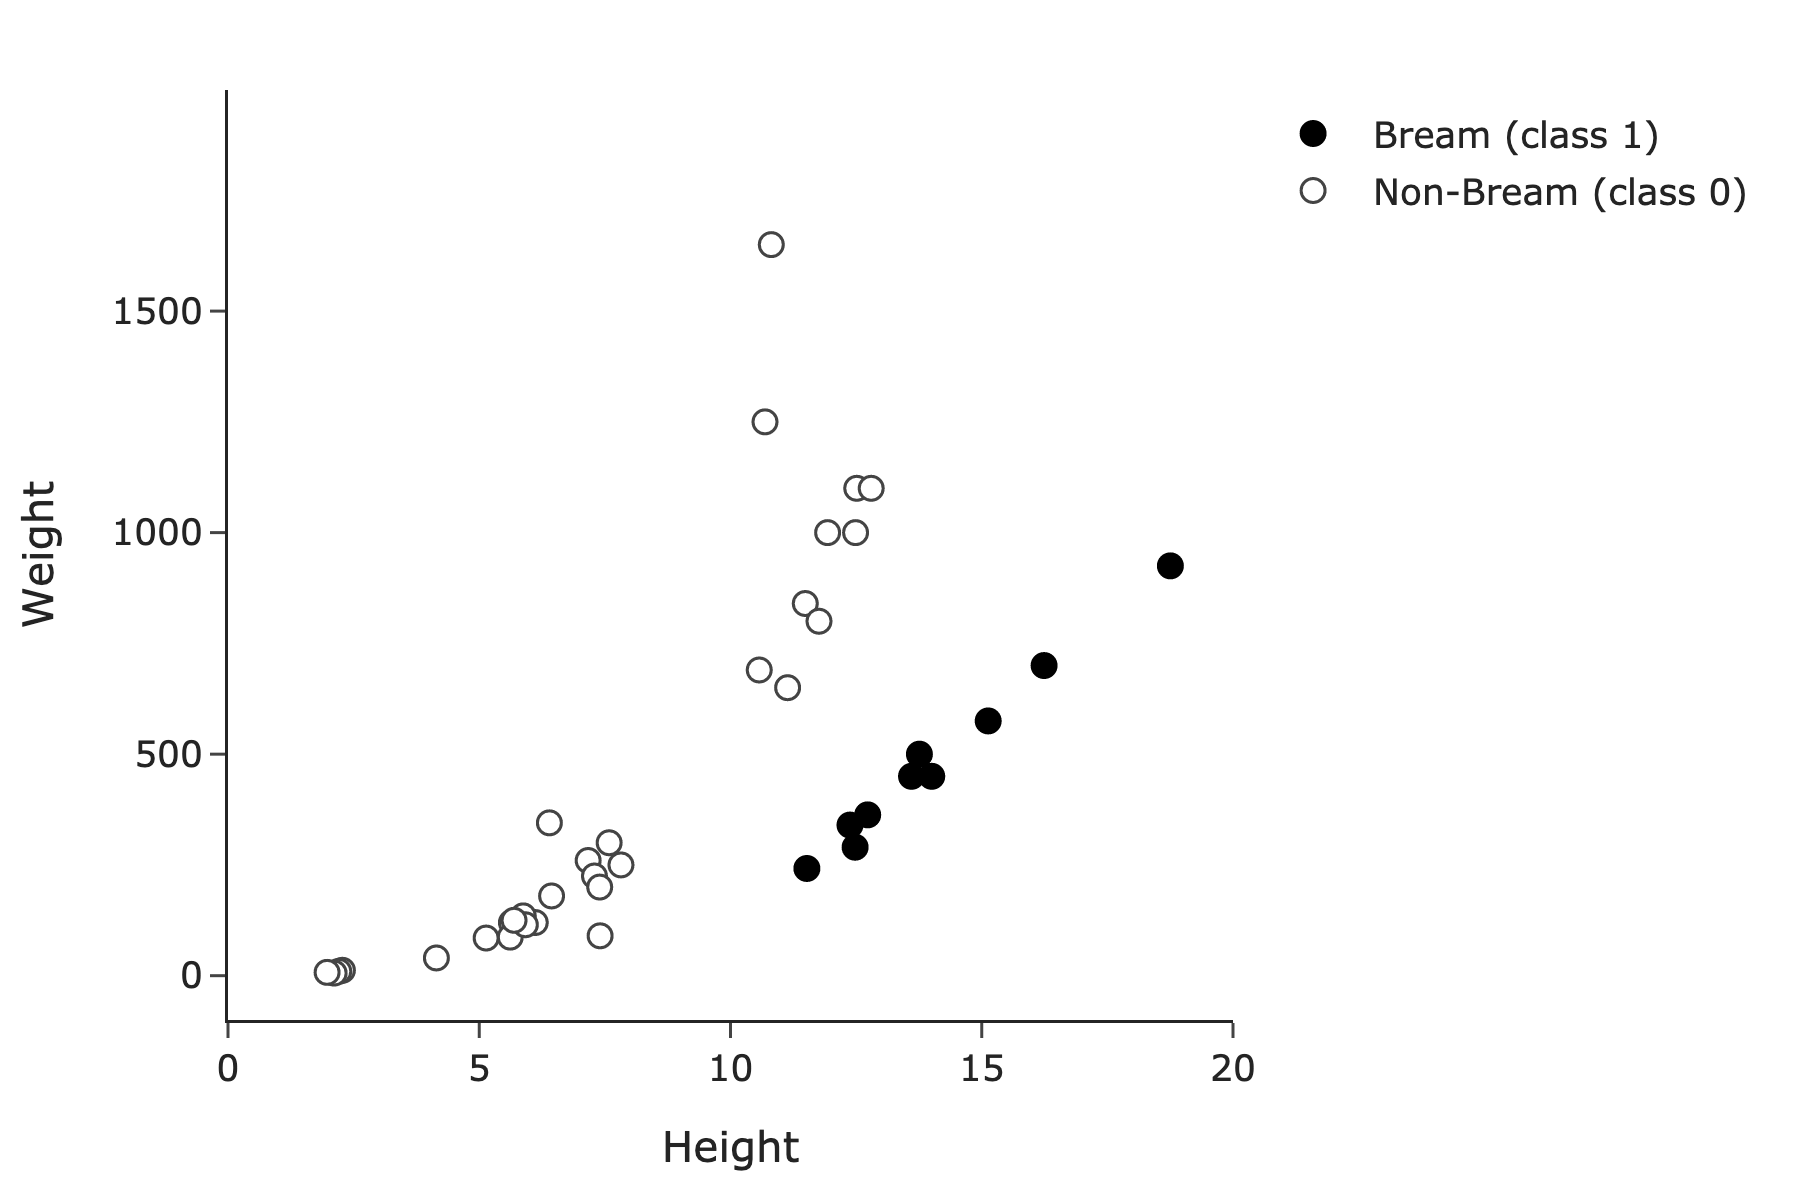
\includegraphics[width=0.8\textwidth]{final-images/scatter-base.png}
\end{center}

\begin{subprobset}

\begin{subprob}(3 pts) Suppose we use height ($x_i$) \textbf{only} to predict species. If we use logistic regression without regularization, which option best describes the fit model, $P(y_i = 1 | x_i)$?

\bubble{$P(y_i = 1 | x_i) = \sigma \left(-15 - \frac{2}{3}x_i \right)$}

\bubble{$P(y_i = 1 | x_i) = \sigma \left(-15 + \frac{2}{3}x_i \right)$}

\bubble{$P(y_i = 1 | x_i) = \sigma \left(-20 + \frac{2}{3}x_i \right)$}

\bubble{$P(y_i = 1 | x_i) = \sigma \left(-15 - \frac{5}{4}x_i \right)$}

\bubble{$P(y_i = 1 | x_i) = \sigma \left(-15 + \frac{5}{4}x_i \right)$}

\bubble{$P(y_i = 1 | x_i) = \sigma \left(-20 + \frac{5}{4}x_i \right)$}

\end{subprob}

\vspace{0.2in}

\begin{subprob}(3 pts) Suppose we use height ($x_i$) \textbf{only} to predict species. If we use $L_2$-regularized logistic regression with a regularization hyperparameter of $\lambda = 10^{10}$, what is the value of $w_0^*$ in the fit model $P(y_i = 1 | x_i) = \sigma(w_0^* + w_1^*x_i)$?

\begin{tabular}{llll}

\bubble{$3$}
& \bubble{$1 / 3$}
& \bubble{$4$}
& \bubble{$1 / 4$} \\

\bubble{$\log \left( 3 \right)$} 
& \bubble{$\log \left( 1 / 3 \right)$}
& \bubble{$\log \left( 4 \right)$}
& \bubble{$\log \left( 1 / 4 \right)$} \\

\end{tabular}
  

% $w_0^* = $ \biginlineresponsebox[1.75in]{} \hspace{0.75in} $w_1^* = $ \biginlineresponsebox[1.75in]{}
    
\end{subprob}
    
\end{subprobset}

\newpage

For the rest of this question, suppose we use \textbf{both} height and weight to predict species. Suppose we use logistic regression --- possibly with regularization --- and choose a classification threshold of $T$, where $0 \leq T \leq 1$. The resulting decision boundary is shown below, along with the same training set as before (which has $n=40$ points, 10 of which belong to class 1).

% Suppose we use logistic regression, potentially with regularization. Once we find optimal parameters $\vec w^*$, we apply a threshold, $T$, where $0 \leq T \leq 1$, which allows us to classify fish as follows:

% $$\text{predicted class}_i = \begin{cases} 1 & P(y_i = 1 | \vec x_i) \geq T \\ 0 & P(y_i = 1 | \vec x_i) < T \end{cases}$$

% The resulting decision boundary is shown below.

\vspace{-0.25in}

\begin{center}
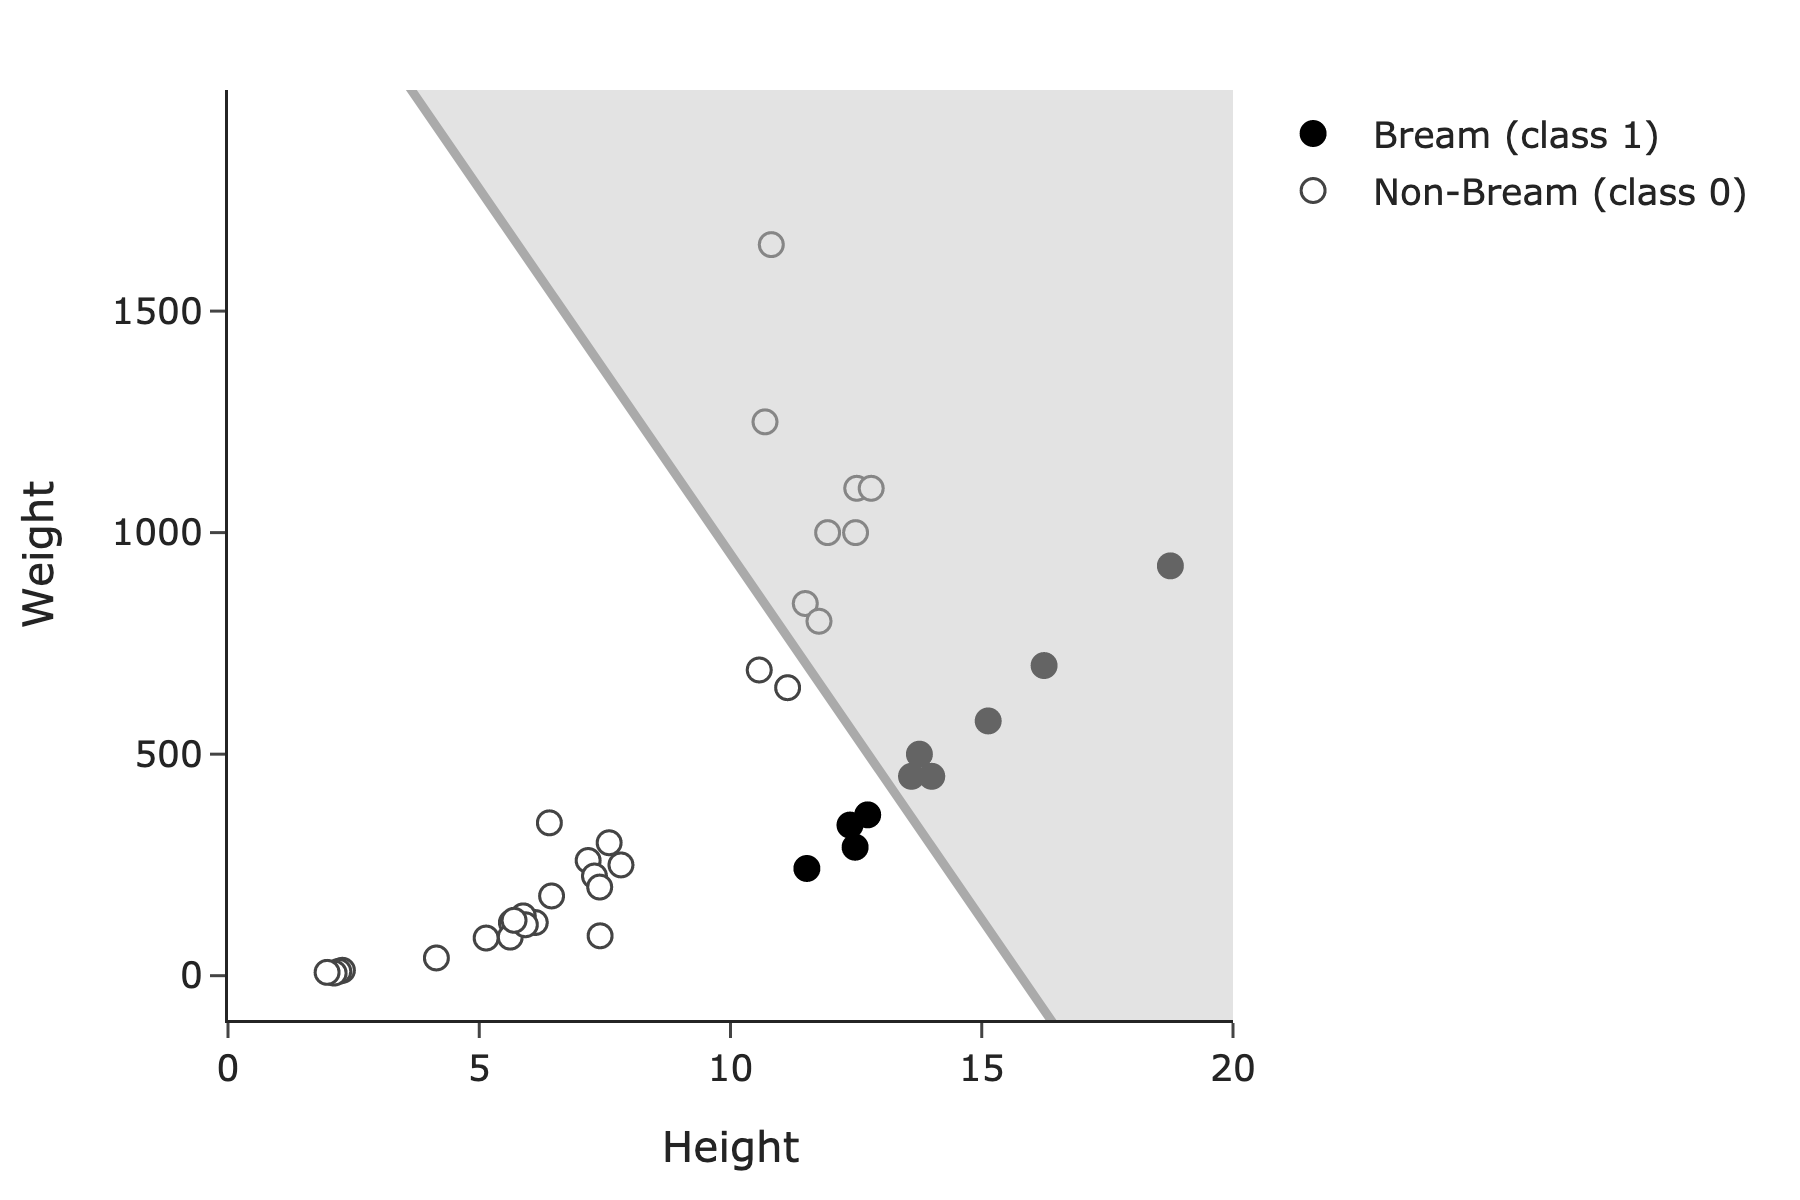
\includegraphics[width=0.8\textwidth]{final-images/scatter-with-boundary.png}
\end{center}

\vspace{-0.1in}

In the region above the line, shaded gray, our classifier predicts class 1 (Bream); in the region below the line, our classifier predicts class 0 (non-Bream).

\begin{subprobset}

\begin{subprob}(2 pts) Was regularization used when fitting the logistic regression model whose decision boundary is shown above?

\bubble{Yes, regularization was used} 

\bubble{No, regularization was not used}

\end{subprob}

\vspace{0.2in}

\begin{subprob}(3 pts) What are the precision and recall of the classifier above? Give your answers as simplified fractions. Answers that ``swap" precision and recall will not be given any credit.

precision = \biginlineresponsebox[2in]{6/14 = 2/7} \hspace{0.4in} recall = \biginlineresponsebox[2in]{6/10 = 3/5}
    
\end{subprob}

\vspace{0.2in}

\begin{subprob}(2 pts) Suppose that each time we accidentally misclassify a fish's species as Bream, we must pay a fine to the local aquarium. Given this fact alone, is it more important for our classifier to have high precision or high recall?

\bubble{High precision} 

\bubble{High recall}
    
\end{subprob}
    
\end{subprobset}

\end{prob}

\newpage

\begin{prob}[(11 pts)]

% 1D clustering

Consider a dataset of $n$ non-negative numbers, $x_1 < x_2 < \ldots < x_n$, that are evenly spaced. In other words, $x_{i+1} - x_i$ is some fixed positive constant, for all $i = 1, 2, ..., n-1$. Furthermore, assume that \textbf{$n$ is an even integer that is not a multiple of 4}.

We'd like to use $k$-means clustering to cluster this dataset into $k = 2$ clusters, Cluster 1 and Cluster 2, defined by two centroids, $\mu_1$ and $\mu_2$, respectively.

Suppose we initialize the two centroids at $\mu_1 = x_1$ and $\mu_2 = x_2$.

\begin{subprobset}

\begin{subprob}(2 pts) In iteration \textbf{1}, \textbf{before} updating the locations of the centroids, how many points belong to each cluster? Give your answers in the form of expressions involving $n$ and/or constants.

Cluster 1: \inlineresponsebox[1.75in]{} \hspace{0.5in} Cluster 2: \inlineresponsebox[1.75in]{}

\end{subprob}

\begin{subprob}(4 pts)  In iteration \textbf{1}, \textbf{after} updating the locations of the centroids, both centroids are located exactly at values in the dataset. Which data point is each centroid now located at? Give your answers in the form of expressions involving $n$ and/or constants, but \textbf{not} $x$. (For example, if you believe $\mu_2$ is now located at $x_{n-1}$, put $n-1$ in the second box.)

\begin{enumerate}[label=(\roman*)]
    \item $\mu_1$ is now located at $x_p$, where $p = \hspace{0.05in} $\inlineresponsebox[1.75in]{}
    \item $\mu_2$ is now located at $x_q$, where $q = $ \inlineresponsebox[1.75in]{}

\end{enumerate}
    
\end{subprob}

\begin{subprob}(3 pts) In iteration \textbf{2}, \textbf{before} updating the locations of the centroids, how many points belong to each cluster? Give your answers in the form of expressions involving $n$ and/or constants.

Cluster 1: \inlineresponsebox[1.75in]{} \hspace{0.5in} Cluster 2: \inlineresponsebox[1.75in]{}

\end{subprob}

\begin{subprob}(2 pts) In one English sentence, name \textbf{and} describe the objective function that $k$-means clustering minimizes.

\begin{responsebox}{1.5in}
    
\end{responsebox}
    
\end{subprob}

% \begin{subprob}

% Where should we place centroids $\mu_1$ and $\mu_2$ in order to minimize inertia for $k = 2$ and this dataset? Give your answers in the form $x_\text{exp}$, where $\text{exp}$ is replaced with an expression involving $n$ and/or constants. There are two possible pairs of answers; provide the answer where $\mu_1 < \mu_2$.

% $\mu_1$: \inlineresponsebox[1.75in]{} \hspace{0.5in} $\mu_2$: \inlineresponsebox[1.75in]{}
    
% \end{subprob}
    
\end{subprobset}


% Fill in the blanks to complete the sentence below.

% The iterative algorithm for $k$-means clustering presented in lecture aims to find the centroids that minimize the squared distance from each point to its closest centroid, \_\_(i)\_\_, and \_\_(ii)\_\_.

% \begin{enumerate}[label=(\roman*)]
%     \item \bubble{averaged separately for each cluster, and then summed for every cluster} \\
%           \bubble{summed across the entire dataset}
%     \item \bubble{always finds the global minimum} \\ 
%           \bubble{may only find a local minimum, depending on the choice of initial centroids} \\
%           \bubble{many only find a local minimum, depending on the choice of learning rate} \\
%     \bubble{may never converge, depending on the choice of initial centroids} \\ 
% \end{enumerate}

\end{prob}

\vspace{0.5in}

\newpage

\textbf{Make sure you've written your uniqname in the space provided in the top right corner of every page of this exam!}

Congrats on finishing the course --- we'll miss you! Feel free to draw us a picture about EECS 398 below :)

% (1 pt) And here's a free point!

\begin{responsebox}{7in}
    
\end{responsebox}

\end{probset}

\end{document}
